\documentclass[border=2pt]{standalone}
\usepackage{tikz}
\begin{document}
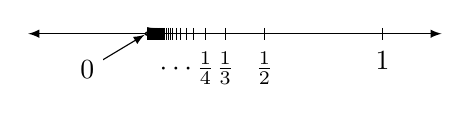
\begin{tikzpicture}[scale=3]
  \draw[latex-latex] (-.5,0) -- (1.25,0);
  \foreach \n in {1,2,...,600}{
    \draw[ultra thin] (1/\n, .025) -- (1/\n, -.025);
    % \node[circle, draw=black, fill=white, inner sep=.5pt] (\n) at (1/\n, 0) {};
    % \node[below] () at (1/\n, 0) {$\frac{1}{\n}$};
  }
  \node[below, yshift=-3pt] () at (1,0) {$1$};
  \foreach \n in {2,3,...,4}{
    % \node[circle, draw=black, fill=white, inner sep=.5pt] (\n) at (1/\n, 0) {};
    \node[below, yshift=-3pt] () at (1/\n, 0) {$\frac{1}{\n}$};
  }

  \node[below,yshift=-7pt] (dots) at (.125,0) {$\cdots$};

  \node[circle, fill=white, draw=black, inner sep=0pt] (zero) at (0,0) {};

  \draw[-latex] (-.25, -.15) -- (zero) node[at start, fill=white] {$0$};

\end{tikzpicture}
\end{document}
